\section{Metabolites in a DesignGG experiment}
\label{sect:Metabolites}
A complex phenotype such as seed germination is the resultant of several genetic and environmental 
cues and requires the concerted action of many genes. The use of well-structured recombinant inbred 
lines in combination with omics analysis can help to disentangle the genetic basis of such 
quantitative traits. This so called genetical genomics approach can effectively capture both 
genetic (G) and epistatic interactions (G:G). However, to understand how the environment interacts 
with genetic information (G:E) a better understanding of the perception and processing of 
environmental signals is needed. In a classical genetical genomics setup this requires replication 
of the whole experiment in different environmental conditions. A novel generalized setup overcomes 
this limitation and includes environmental perturbation within a single experimental design. 

We developed a dedicated QTL mapping procedure to implement this approach and used existing 
phenotype data to demonstrate its power. Additionally, we studied the genetic regulation of 
primary metabolism in dry and imbibed Arabidopsis seeds. Many changes were observed in the 
metabolism which are both under environmental and genetic control and their interactions. 
This concept offers unique reduction of experimental load with minimal compromise of statistical 
power and is of great potential in the field of systems genetics which requires a broad 
understanding of both plasticity and dynamic regulation.

\subsection{Background}
The use of natural variation to disentangle the genetic \del{(G)} mechanisms underlying differences in phenotypes 
has been very successful both in crop plants and in the model plant Arabidopsis (Arabidopsis thaliana\rev{)}; 
\cite{Alonso-Blanco:2009}. Most of the variation within wild or domesticated plant species is of 
quantitative nature determined by \rev{genetic} polymorphisms at multiple loci. Such quantitative trait loci (QTL) 
can be analyzed efficiently using experimental mapping populations such as recombinant inbred lines (RILs)
derived from directed crosses. Nowadays, many well structured RIL populations are available, often 
accompanied with detailed studies of phenotypic variation \cite{Mitchell-Olds:2006}. The complexity 
of quantitative traits is further determined by the interactions between genomic loci (i.e. epistasis) and 
between the genotype and the environment (genetic X environmental [G:E]). While epistasis can be effectively
identified in QTL analyses, albeit with lower power than main effects, the detection of G:E interactions 
requires experimentation in multiple conditions of interest. Because of the large population sizes often 
needed to obtain sufficient statistical power for QTL detection, G:E interactions are usually ignored in 
experimental setups. However, a better understanding of the perception and processing of environmental (E)
signals is greatly needed, because interactions provide important insights in adaptation mechanisms and
evolutionary constraints such as balancing and disruptive selection. To obtain a more detailed view of the
molecular mechanisms underlying phenotypic variation, genetical genomics studies, in which molecular traits
are genetically analyzed, have been successfully applied to enhance a directed strategy to identify causal
relationships \cite{West:2007, Keurentjes:2007, Kliebenstein:2006, Rowe:2008}. The observed phenotype is often the resultant 
of a functional cascade of gene transcription followed by protein translation and modification, which 
finally leads to a highly dynamic metabolome underlying emergent properties \cite{Kooke:2012}. 
With the technological advances made in genomic analytical platforms, such as transcriptomics, proteomics, 
and metabolomics, the large-scale, high-throughput analyses needed for quantitative \rev{genetic} approaches have 
become feasible \cite{Jansen:2001a}. 

Incorporating developmental and \rev{environmental} perturbation in the often expensive and laborious omic analyses, an 
alternative experimental setup, coined \rev{'}generalized genetical genomics\rev{'} (GGG), using balanced fractions 
of a RIL population has been proposed \cite{Li:2009}. It provides a cost-effective experimental setup 
for hypothesis-generating research in multiple environments. Such an approach aims for the creation of 
subpopulations of RILs, one for each environment to be tested, with an optimal distribution of parental 
alleles over all available markers \cite{Li:2009}. When these subpopulations are subjected to \rev{environmental} 
perturbation, the emerging phenotypes can be explained by several sources of variation: \rev{Genetic} variation, 
\rev{Environmental} variation, and G:E variation. Whenever the resulting phenotype is not or only mildly affected by \del{E} 
interactions (G:E), the analysis of the different subpopulations can be combined, gaining the full power 
of a complete population. However, when a trait shows strong G:E interaction (e.g. those that only express 
\rev{genetic} variation in specific environments), the power to detect QTL is dependent on those subpopulations 
expressing the \rev{genetic} variation. Although G:E interactions have been detected previously in genetical 
genomics studies for expression \cite{Li:2006, Smith:2008, Gerrits:2009} and metabolite content 
\cite{Zhu:2012} by analyzing all lines in a population under different environments, the GGG concept 
offers an effective way of studying a combination of \rev{genetic} and \rev{environmental} perturbations and is of great potential 
in the field of systems genetics, in which a broad understanding of both plasticity and dynamics is 
required \cite{Li:2008}. The fundamental basis of the experimental design and data analysis using a 
full model ($Y = E + G + G:E + e$), where $Y$ is the observed phenotype and $e$ is residual error, 
is generally valid and frequently used \cite{Churchill:2002, Li:2006,Gerrits:2009}. As a proof of 
principle, we present experimental data on the \rev{genetic} regulation of primary metabolism in dry and imbibed 
Arabidopsis seeds using a GGG design and discuss the application and implications of such a strategy.

Plants are extremely rich in biochemical compounds, and major roles in plant development, adaptation, 
and defense have been identified for biosynthesis pathways and their products (Binder, 2010). The 
biosynthetic pathways of primary metabolites are well studied and often well conserved between 
different taxa \cite{Peregrin-Alvarez:2009}. Nonetheless, quantitative variation for many of 
these compounds can be observed between natural variants, which might be reflected in their different 
growth characteristics. The analysis of single-gene mutants, for example, has unraveled many key 
components in biochemical pathways and has demonstrated their role in phenotypic traits 
\cite{Fiehn:2000}. In Arabidopsis, \rev{genetic} variation for many of its metabolic compounds has been 
observed \cite{Kliebenstein:2001, Rowe:2008, Keurentjes:2006}, but G:E interactions 
were ignored in these studies and only addressed by Chan et al. \cite{Chan:2011}. Metabolic profiling at different 
growth stages has further revealed important fluxes that regulate plant development and adaptation 
\cite{Oliveira:2010}. Using the accumulated historical mutations that occur in natural 
variants in combination with metabolic profiling in a generalized design offers the unique possibility 
of identifying G effects over a series of developmental stages. Here, we report on the interaction of 
four different physiological environments (i.e. developmental stages) in dry and imbibed seeds with 
two founder genotypes in a RIL population. To detect the majority of the most prominent primary 
metabolites, we used gas chromatography-mass spectrometry of polar extracts \cite{Roessner:2000, 
Lisec:2008}. These include essential metabolites such as sugars, amino acids, and organic 
acids, which are key compounds in reserve storage and catabolism, growth, and energy metabolism.

The switch from a dry seed, which is equipped for optimal survival and storage of reserves, toward an
imbibed seed, in which energy needed for germination is released and which prepares for autotrophic 
production, is remarkable. Reserves that have been stored during seed maturation are degraded and remobilized
during germination \cite{Bewley:1997,Shu:2008}, a process that is heavily influenced by the capacity 
of carbon/nitrogen partitioning of a maturing seed \cite{Dowdle:2007}. Arabidopsis mutants affected 
in their oil reserve content or its mobilization show delayed but not full inhibition of germination 
\cite{Kinnersley:2000, Bouche:2004, Shu:2008, Kelly:2011}. This suggests 
an additional metabolic switch that occurs during seed desiccation after seed maturation involving a change 
from accumulation of oil and storage proteins to the synthesis of free amino acids, sugars, fatty acids, 
and their degradation products functioning to prepare for rapid metabolic recovery during imbibition 
\cite{Fait:2006, Angelovici:2010}. Imbibition of mature seeds specifically shows reduction of 
the metabolites that accumulate during the desiccation period. Upon germination, an increase of many 
metabolites, including amino acids, sugars, and organic acids, can be observed again, which reflects 
the increase of autotrophic activity \cite{Fait:2006}. Profiling the primary metabolome over different 
developmental stages in a mapping population is therefore expected to reveal the dynamics of \rev{genetic} regulation 
of many of these important processes. We will demonstrate here that much of the observed variation in 
biochemical profiles can be attributed to genotype-by-environment interactions, which can be effectively 
identified in a GGG approach.

\subsection{Results}

\subsubsection{Experimental Design}
Previous studies which focused on the comparative analysis of developmental and metabolic variation suggest 
a link between central metabolism and plant physiology, but genetic co-regulation is not frequently observed 
\cite{Keurentjes:2006, Meyer:2007}.  That said, in several studies in Arabidopsis a major 
metabolite QTL cluster is associated with the ERECTA locus, representing a strong regulator of development 
which is known for its pleiotropic effects (Fu:2009). To circumvent this strong bias we used two 
natural variants, Bayreuth-0 (Bay-0) and Shahdara (Sha), which are not polymorphic for the ERECTA locus. 
The Bay-0 x Sha RIL population \cite{Loudet:2002} has previously been shown to contain genetic variation 
for seed germination \cite{Joosen:2011} and other physiological traits \cite{Loudet:2003a, Barriere:2005, 
Loudet:2005, Diaz:2006, Reymond:2006, Loudet:2008, Meng:2008}, anion strength 
\cite{Loudet:2003a}, carbohydrate content \cite{Calenge:2006}, gene expression \cite{West:2007} and primary 
\cite{Rowe:2008} and secondary metabolite levels \cite{Wentzell:2007}. 

Powerful mapping of genetic variation in a RIL population is dependent on the size of the population, the level 
of recombination and on an evenly genome-wide distribution of the parental alleles. In the present study, a core 
set of the Bay-0 x Sha RIL population \cite{Loudet:2002} consisting of 165 lines and optimized for the 
aforementioned factors used. This core population was carefully divided in four sub-populations optimized for 
the distribution of parental alleles using the R-package DesignGG, aiming at the most accurate estimate of genetic 
effect and G:E effect \cite{Li:2009}.

\subsubsection{Comparison of Different Designs Using Classic Phenotypes}
Standard QTL mapping procedures can efficiently capture genetic variation and epistasis, but do not take 
environmental perturbation into consideration. Appropriate modeling of the genetic variance-covariance (VCOV) 
in the data is of great importance when combining information from different environments in QTL analysis 
\cite{Churchill:2002}. Linear models are particularly well suited for this. Here environmental differences are 
incorporated as an additional variable in a generalized design (GGG design). To enable mapping of the observed 
trait variation and taking the four developmental stages into consideration an R-script was developed which use 
functions and data structures from the R/qtl package \cite{Broman:2003, Arends:2010}.
The R-script uses a linear model to calculate the likelihood of genotype to phenotype linkage for each marker 
with the following formula:

$$ y_{i}   =   \beta_{0} + \beta_{1}e_{i} + \beta_{2}g_{i} + \beta_{3}g_{i}:e_{i} + \epsilon_{i} $$

Where $y_{i}$ is the ith observation of the studied phenotype, variable $g_{i}$ is the genotype, $e_{i}$ is a vector with seed 
conditions, and $e_{i}:g_{i}$ the interaction term. The values βj represent parameters to be estimated, and $\epsilon_{i}$ is the 
error term. The simplified description $Y = E + G + G:E + \epsilon$ of this linear model will be used henceforward. Separate 
likelihood estimates (-log10 Probability, henceforth LOD scores) are generated for the environmental (E), genetic 
(G) and genetic x environmental (G:E) effects. 

To validate the use of a GGG design, we studied the genetic (G) and the interacting effects 
between \rev{genetics} and \rev{environment} (G\rev{:}E) on phenotypes in four different environmental conditions (E). These 
phenotypes were obtained by studying different germination parameters under different environmental 
conditions \cite{Joosen:2011}. In total we compared the power of different designs by performing 
QTL analysis for 96 classic phenotypes under 4 different environments \cite{Joosen:2011} (table \ref{table:designs}).  
Furthermore, we also investigate the interacting effect between genotype and environmental. The full model 
mapping ($Y = E + G + G:E + \epsilon$) was applied to full block design, random design and GGG design. 
Single maker mapping ($Y = G + \epsilon$) was applied to single block design. The number of detected QTL and interacting 
QTL (FDR = 0.05, based on >10000 runs permutation) with the different designs are shown in the Table \ref{table:designs}.  
In the \rev{full} block design\rev{,} all samples were allocated to the four conditions. Obviously, this is the most expensive way of performing 
the experiment as the required resources and effort is quadrupled (4 x N). As a result of the size of the experiment, 
the power of detecting genetic effects is the best for this design. Unfortunately, we cannot afford such expensive 
experiments in many situations due to limited resource and time. The single block design only focuses on one of the four 
conditions, as in most published genetical genomics studies to date. In this way the effect samples size for the selected 
condition is N and we will have equal power as full block design for detecting the genetic effects for this particular 
condition. Clearly, this design will miss the information from the other three conditions and interacting effects 
between genetic and environmental factors cannot be investigated. In order to study both genetic and interacting 
effects with a limited budget, the random and the GGG design allocate the N different samples to the four environments 
evenly, measuring N/4 samples in each condition. Although the possibility to detect genetic effects is only slightly better 
for the GGG design, the detection of interacting QTL is clearly improved in the GGG design as compared to the random design. 
These results show that the optimal allocation of samples as in the GGG design clearly improves the ability to detect both 
genetic and interacting effects and that the GGG design results in the maximisation of detected variation in relation to 
the necessary resources with only a minimal compromise of statistical power as compared to the full block design.

\begin{table}[!ht]
  \begin{center}
  {\footnotesize
  \begin{tabular}{ l  c  c }
    \hline
    {\bf Design} & {\bf QTL} & {\bf Interacting QTL}\\
    \hline
    Full-Block     & 96     & 30\\
    \ \ \ Best power for G effect & &\\
    \ \ \ Most expensive & &\\
    \ \ \ Best power for G:E effect & &\\

    Single-Block   & 93     & 0\\
    \ \ \ Same power for G in selected condition & &\\
    \ \ \ Less expensive & &\\
    \ \ \ Missing G:E effect & &\\
    Random         & 78(75) & 17(5)\\
    \ \ \ Limited power G effect & &\\
    \ \ \ Less expensive & &\\
    \ \ \ Limited power G:E effect & &\\
    DesignGG       & 81(67) & 27(12)\\
    \ \ \ Optimal power for G effect & &\\
    \ \ \ Less expensive & &\\
    \ \ \ Optimal power for G:E effect & &\\
    \hline
  \end{tabular}
  }
  \end{center}
  \caption[Comparing different experimental designs]{Comparison of different experimental designs to study G and G:E effects 
  		  on classic phenotypes in four different conditions. Each E condition is indicated with different gradient of gray 
  		  in the blocks. In total there are n (164) genetically different RILs, and the data were analyzed in four different 
  		  ways. The last two rows compare the number of QTLs for main G effect and G:E interacting effect detected using 
  		  different design strategies. The numbers in parentheses indicate the QTLs that share confidence intervals (1.5 
  		  drop-off) with the full-block design.}
    \label{table:designs}
\end{table}

\subsubsection{Metabolic Analysis}
To study the metabolic status of Arabidopsis seeds during germination, four biologically important developmental stages 
of seed germination with expected variation in metabolite levels to different extent were selected. The first two stages, 
being freshly harvested primary dormant (PD) and after ripened (AR) non-dormant dry seeds, respectively, are expected to 
comprise a very similar metabolome as most, if not all, metabolic fluxes are arrested in the dry seed. The oil rich 
(\textasciitilde40\%) Arabidopsis seeds \cite{Hobbs:2004} typically desiccate to moisture contents below 5\% which results in an 
arrest of all enzymatic reactions due to the lack of free water. The other two stages represented early imbibition of 
seeds, imbibed for 6 hours (6H), and seeds at radical protrusion (RP), respectively. Full rehydration of dry seeds typically 
completes in less than 2 hours and although developmental differences are not yet expected, many metabolic processes will 
have started after 6 hours of imbibition \cite{Nakabayashi:2005, Howell:2009}. Radicle protrusion marks the end-
point of germination sensu stricto and is known to be accompanied by a major switch of both the transcriptome and metabolome 
\cite{Nakabayashi:2005, Fait:2006}. These four developmental stages are anticipated to vary to different degrees 
in their metabolic profiles, hardly any difference between dry seed samples, some differences between dry and imbibed seeds 
and very pronounced differences between dry seeds and seeds at radicle protrusion.

To determine the metabolic status of genetic variants in these different developmental stages, all individuals in the 
four sub-populations and their parental accessions were subjected to GC-TOF-MS. Each sample consists of the polar fraction 
of a methanol extract of a bulk of approximately 700-1000 seeds (20 mg). Samples were analyzed in random order and 
interspersed with pooled sample controls to control for experimental errors. The metabolic profiling of the segregating RILs 
was performed and the use of segregation population provides an intrinsic replication for each genotypic marker \cite{Jansen:2001a}.
In total 7537 mass peaks were detected, representing 161 metabolites according to centrotyping based on retention time and 
correlation structure \cite{Tikunov:2012}. In total 63 metabolites could be annotated using an in-house constructed library 
and a publicly available mass spectra library \cite{Schauer:2005}. Parental accessions were measured in duplicate for all 
four developmental stages allowing us to model the influence of condition and accession using a multi-factor univariate 
analysis of variance (ANOVA). 

$$ y_{i}   =   \beta_{0} + \beta_{1}condition_{i} + \beta_{2}accession_{i} + \epsilon_{i} $$

Analysis of variance for the parental samples identified 108 metabolites showing significant variation (FDR < 0.05) between 
developmental stages (E) and 85 showing variation between the parents (G) with an overlap of 54 metabolites showing variation 
between both variables in an interactive way (G:E) (Supplemental file 2). For 37 metabolites no significant variation was 
detected between the parental accessions or in any of the developmental stages. A self-organizing map (SOM), created from the 
metabolites showing significant variation between the parents, groups different metabolites according to their accumulation 
pattern over different genotypes and developmental stages (Fig. \ref{fig:SOM}). Clearly different patterns of variation can be observed, 
namely genetic in panel A and H; environmental in panel C and D; genetic + environmental in panel B and G and genetic x 
environmental in panel E and F, illustrating the complex regulation of metabolic processes and the need for sophisticated 
analysis methods, like PCA or Multiple QTL mapping\cite{Arends:2010}. 

\begin{figure}[!ht]
  \centering
  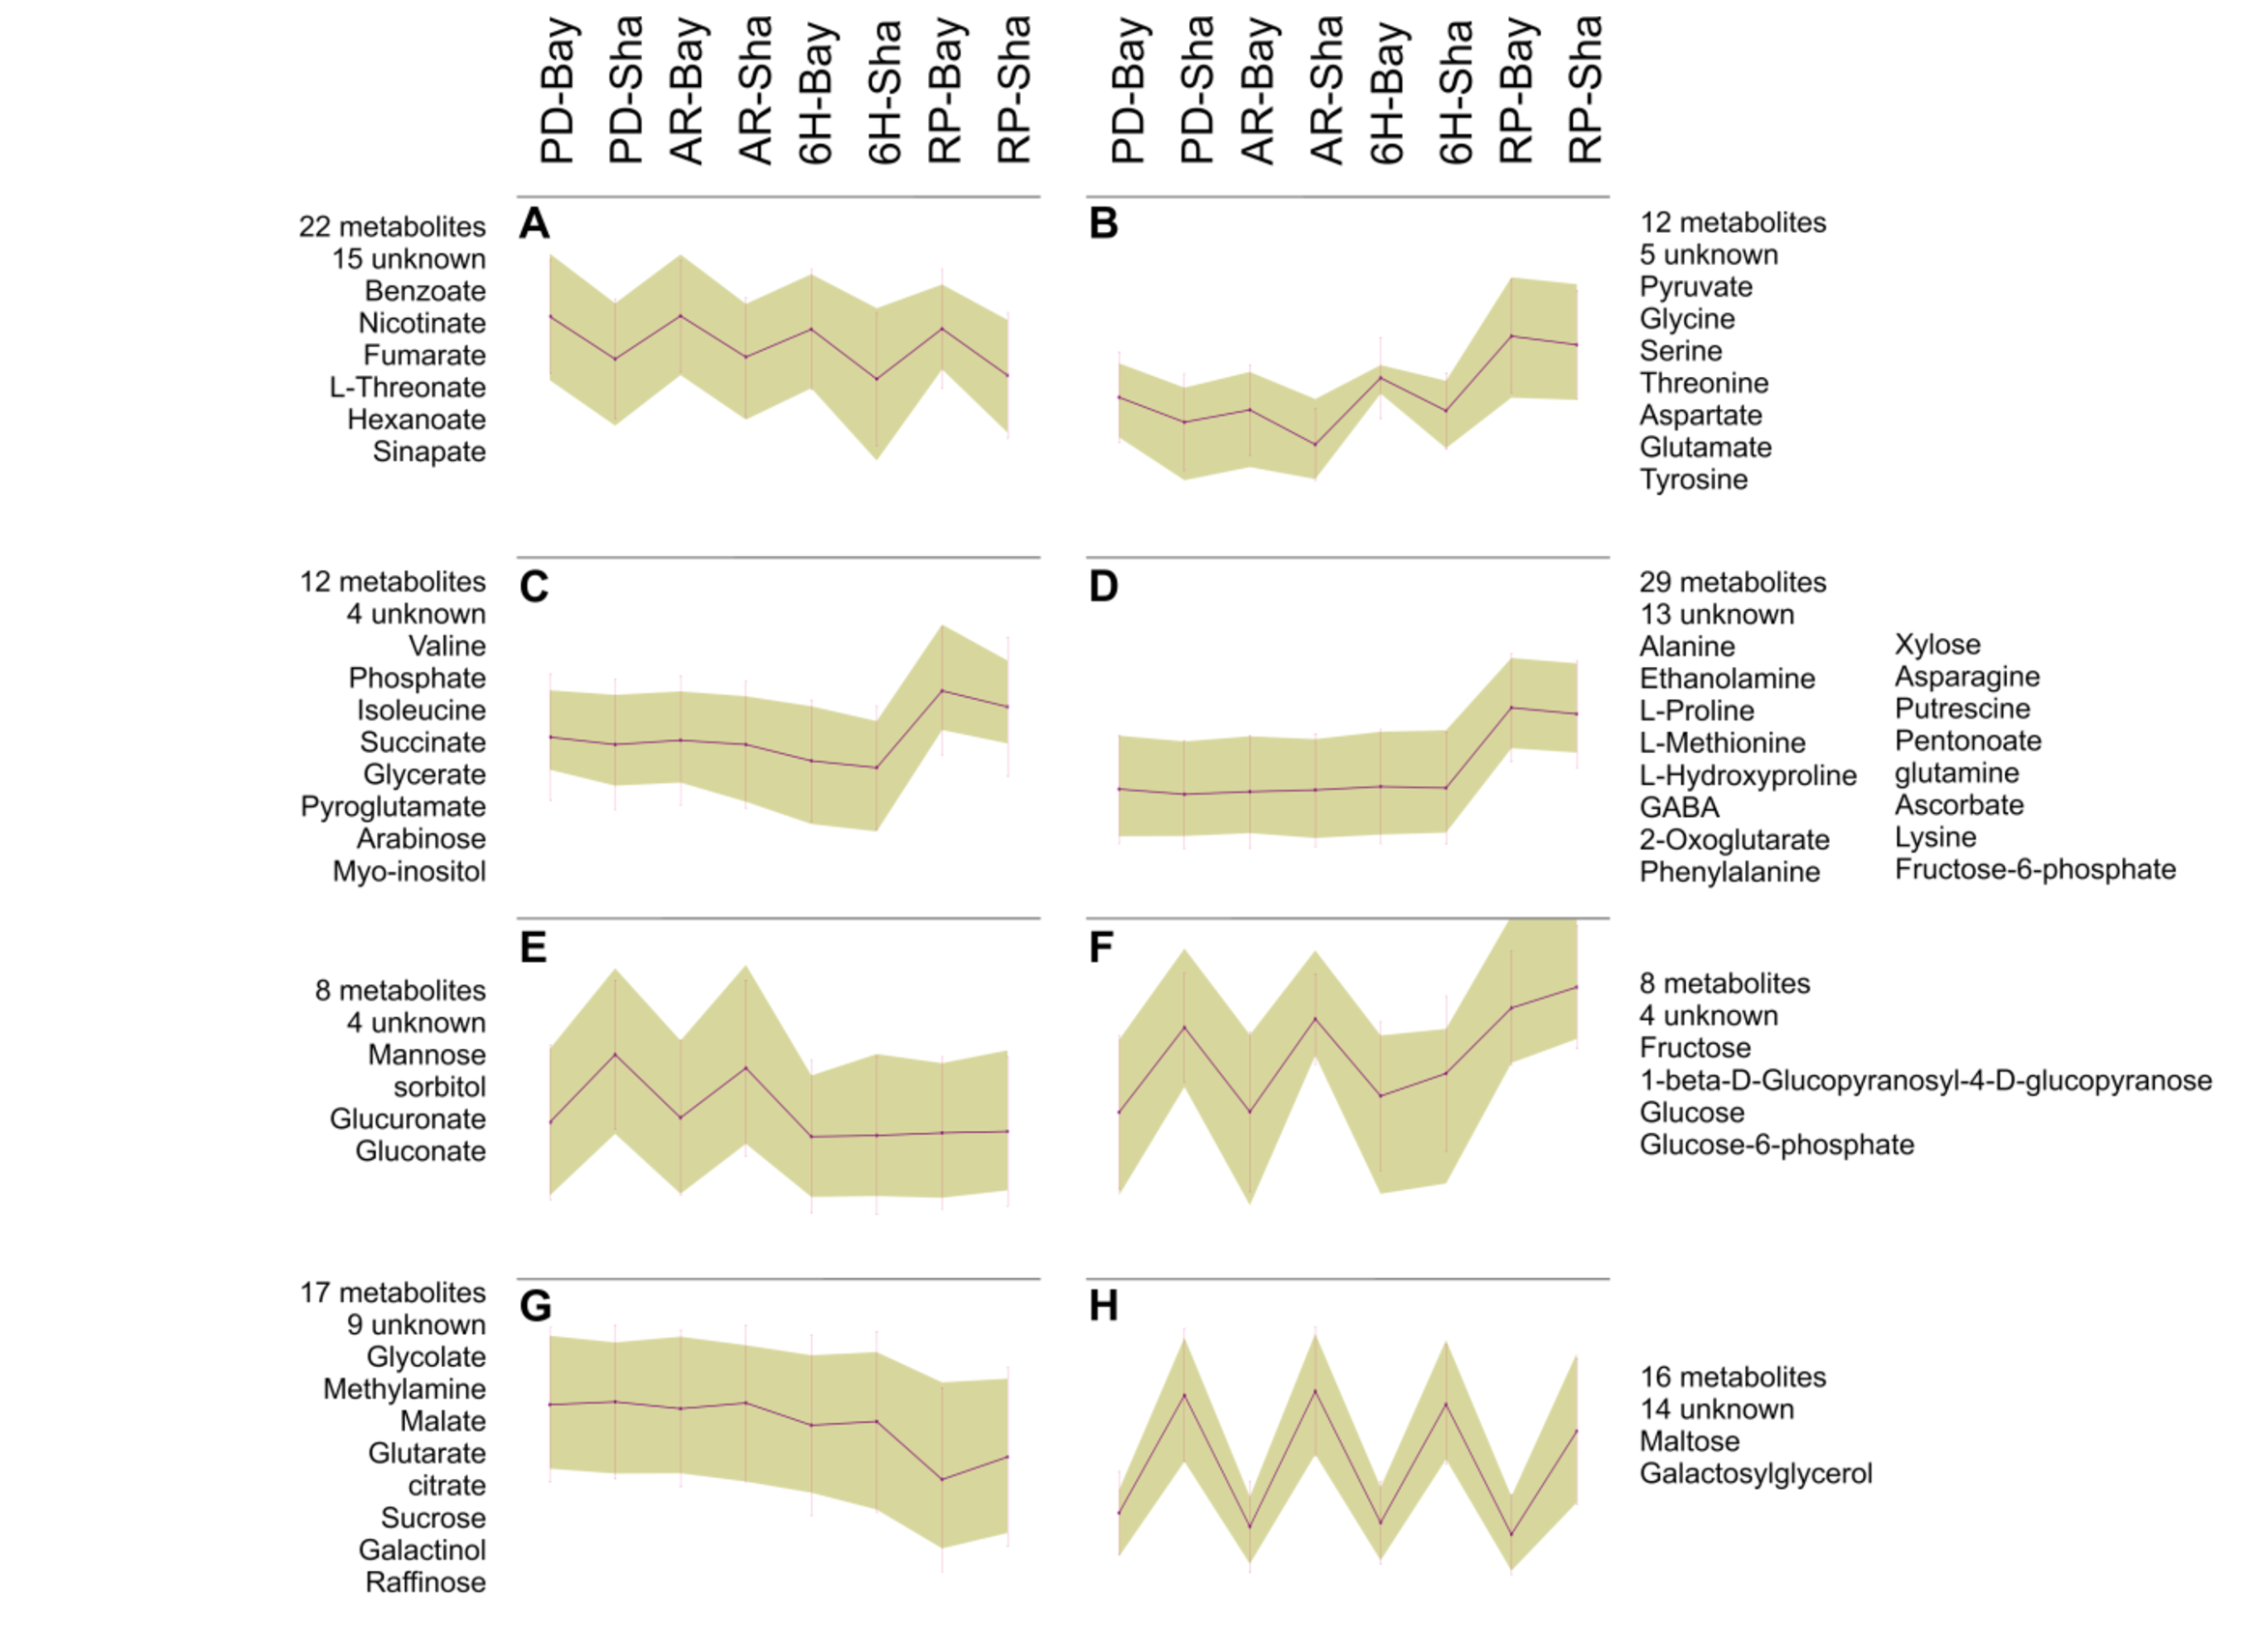
\includegraphics[keepaspectratio,scale=0.30]{eps/image_3_2_1.eps}
  \caption[Self organizing map]{Self organizing map, grouping different metabolites according to their accumulation pattern over different 
    genotypes and developmental stages of significantly variable metabolites (anova F pr. < 0.05)  measured in the parental lines Bay-0 
    and Sha in four developmental stages.  PD=Primary dormant, AR=After-ripened, 6H=6 hour imbibed, RP=seeds at radicle protrusion. Two
    independent biological replicates were measured for each combination of parent and developmental stage.}
    \label{fig:SOM}
\end{figure}

Because metabolite levels are varying between both parents and between the chosen seed germination stages, a segregation of 
metabolic accumulation can be expected in the RIL population of 164 lines. A principle component analysis of the metabolic 
profiles, revealing the internal structure in the data, shows that the first component clearly separates 6-hour imbibed seeds 
and seeds at radicle protrusion from both primary dormant and after ripened seeds, explaining 37\% of the total variation. 
This confirms the large metabolic changes accompanying the transition from dry arrested seeds to the 
imbibed and germinating developmental stages. As expected, no obvious differences could be detected between the metabolomes 
of primary dormant and after ripened dry seeds. The second component, explaining 11\% of the total variation, sharply separates 
the parental accessions, indicating that this component explains most of the genetic variation in metabolic profiles. These 
results demonstrate that Bay-0 and Sha possess substantial genetic variation for the accumulation of primary metabolites which 
segregates in their recombinant offspring and which is strongly influenced by the developmental stage used for profiling.

Transgressive segregation \rev{(when the expression of the offspring exceeds the expression of the parents)} was visualized 
by comparing parental and RIL metabolite level distributions (Fig. \ref{fig:transgression}). 
Some positive and negative transgression is observed for most of the metabolites in which the metabolite accumulation in a 
RIL is respectively higher or lower compared to the respectively highest or lowest parent. In addition, 15 metabolites were 
detected in RILs which were not present in either parent. This suggests that new allele combinations in the RIL population 
resulted in enhanced accumulation or even novel formation of metabolites.


\begin{figure}[!ht]
  \centering
  \includegraphics[keepaspectratio,scale=0.30]{eps/image_3_2_0.eps}
  \caption[Transgression]{Positive and negative transgression is observed for most of the metabolites in which the metabolite 
  		  accumulation in a RIL is respectively higher or lower compared to the respectively highest or lowest parent.}
    \label{fig:transgression}
\end{figure}


\subsubsection{\rev{QTL} mapping of metabolites in a generalized genetical genomics design}
In the experimental setup of this study, the \rev{environmental} variation is defined as variation observed between the four
developmental stages (PD, AR, 6H, and RP). Significance thresholds, determined by permutation analysis
($n = 1,000, P < 0.01$) for each metabolite, ranged from LOD 3.43 to LOD 3.50 and was stringently set to 
LOD 4 for all analyses. Mapping resulted in 120 significant QTLs in the \rev{genetic} component for 83 metabolites and 
31 G:E QTLs for 27 metabolites, ranging from one to four QTLs per metabolite. Thirteen of the G:E QTLs are
significant in the \rev{genetic} component as well. For 66 metabolites, no significant QTL was detected.

To test the performance of the generalized mapping procedure, QTLs detected in individual environments
using the linear model $Y = G + \epsilon$ were compared with QTLs detected in the combined mapping 
approach (using the linear model $Y = E + G + G:E + \epsilon$; Fig. \ref{fig:qtlComparison}).
QTLs were binned in upper or lower chromosome arms to reduce the effects of small positional shifts.
Results were plotted in a network, with nodes representing QTLs connected with edges to nodes representing 
the mapping populations in which they were detected (Fig. \ref{fig:qtlComparison}). QTLs are grouped in three sections
according to their detection in the different mapping procedures. The middle section shows 73 QTLs that
were detected in both the $Y = E + G + G:E + \epsilon$ model and in one or more single-environment mappings 
using the $Y = G + \epsilon$ model. This shows that most of the G variation present in the single environments 
can effectively be captured by using the generalized model.

The presence of 60 QTLs that were only significantly detected in the $Y = E + G + G:E + \epsilon$ model 
(right section) shows the combined power of the generalized approach and the usage of more genotypes. 
These QTLs are not detected in the single-environment mapping in which only 41 individuals were used.
Combining all data across all environments in the linear model increases power to detect QTLs, but it
should be noted that there are also 20 minor QTLs (left section) that are only significant in the single
environment mapping using the $Y = G + \epsilon$ model. These QTLs are not detected in the $ Y = E + G + G:E + \epsilon$
model. This can be explained by two factors: (1) environments in which the \rev{QTL} is not expressed
introduce noise in the experimental data and thereby decrease mapping power, and (2) deviations from a
balanced allele distribution in the different subpopulations can introduce some stochasticity around the
threshold level, although this is not the case in our data.

Importantly, all major-to-moderate-effect-size QTLs could be detected using the generalized model, even
when these QTLs were not detected in the separate environment models. Although it is difficult to 
compare power with the latter models, because population sizes differ, the generalized design 
efficiently identifies all relevant QTLs, which were detected by the four separate models, and in addition, 
it detects G:E interactions. In a general exploratory study, the reduction in experimental burden therefore 
amply outweighs the incidental failure to detect the limited number of small-effect QTLs. The application 
of a GGG design can thus be an important advancement in evolutionary and ecological studies assessing 
the contribution of \rev{genetic} and \rev{environmental} effects to natural variation in life history traits.

For breeding purposes, the allelic effect size is an important measure, and differentiation of the 
environment in which the allelic effect is expressed can be very useful. In the generalized setup, 
the allelic effect size of those metabolites with significant QTLs is separated per environment 
(Supplemental Files S4 and S5). For every QTL that is consistently detected in all four conditions, 
a LOD score for G effect (Fig. \ref{fig:effectSizes},x axis) is obtained from full-model mapping. For these QTLs,
normalized allelic effect sizes are calculated by Z-score transformations for each environment 
(Fig. \ref{fig:effectSizes}, y axis). QTLs detected \del{in the G component of the linear model} (Fig. \ref{fig:effectSizes}A) show an expected 
linear relationship between LOD score and effect size in all measured environments. This correlation 
is much weaker for QTLs detected in the G:E component of the linear model (Fig. \ref{fig:effectSizes}B) because the \rev{QTL}
 is not expressed in all environments. QTLs of metabolites with strong G:E interaction, 
therefore, display larger effect sizes in fewer environments compared \ref{to} \del{G-component} QTLs of 
similar significance levels \rev{expressed in all conditions}.

Clearly, the choice of environments used in these studies is crucial \cite{Li:2008}. Limited power 
can be expected when environments vary too much and no overlapping G variation is present, and 
contrarily, there is hardly any additive value of the design when using very similar environments. 
In this study, we carefully selected four biologically relevant developmental stages of seed germination 
with expected variation in metabolite levels to different extent and consider them as an \rev{environmental} factor in 
the follow-up statistical analysis. The selected developmental stages start from PD dry seeds to 
seeds at the point of RP. The first two stages, being freshly harvested PD and AR non dormant dry 
seeds, respectively, are expected to comprise a very similar metabolome, as most, if not all, metabolic
fluxes are arrested in the dry seed. The other two stages represent 6H seeds and seeds at RP, respectively.
\del{Different levels of E variation were obtained and could be mapped by the G and/or G:E component of 
the linear model.}

\begin{figure}[!ht]
  \centering
  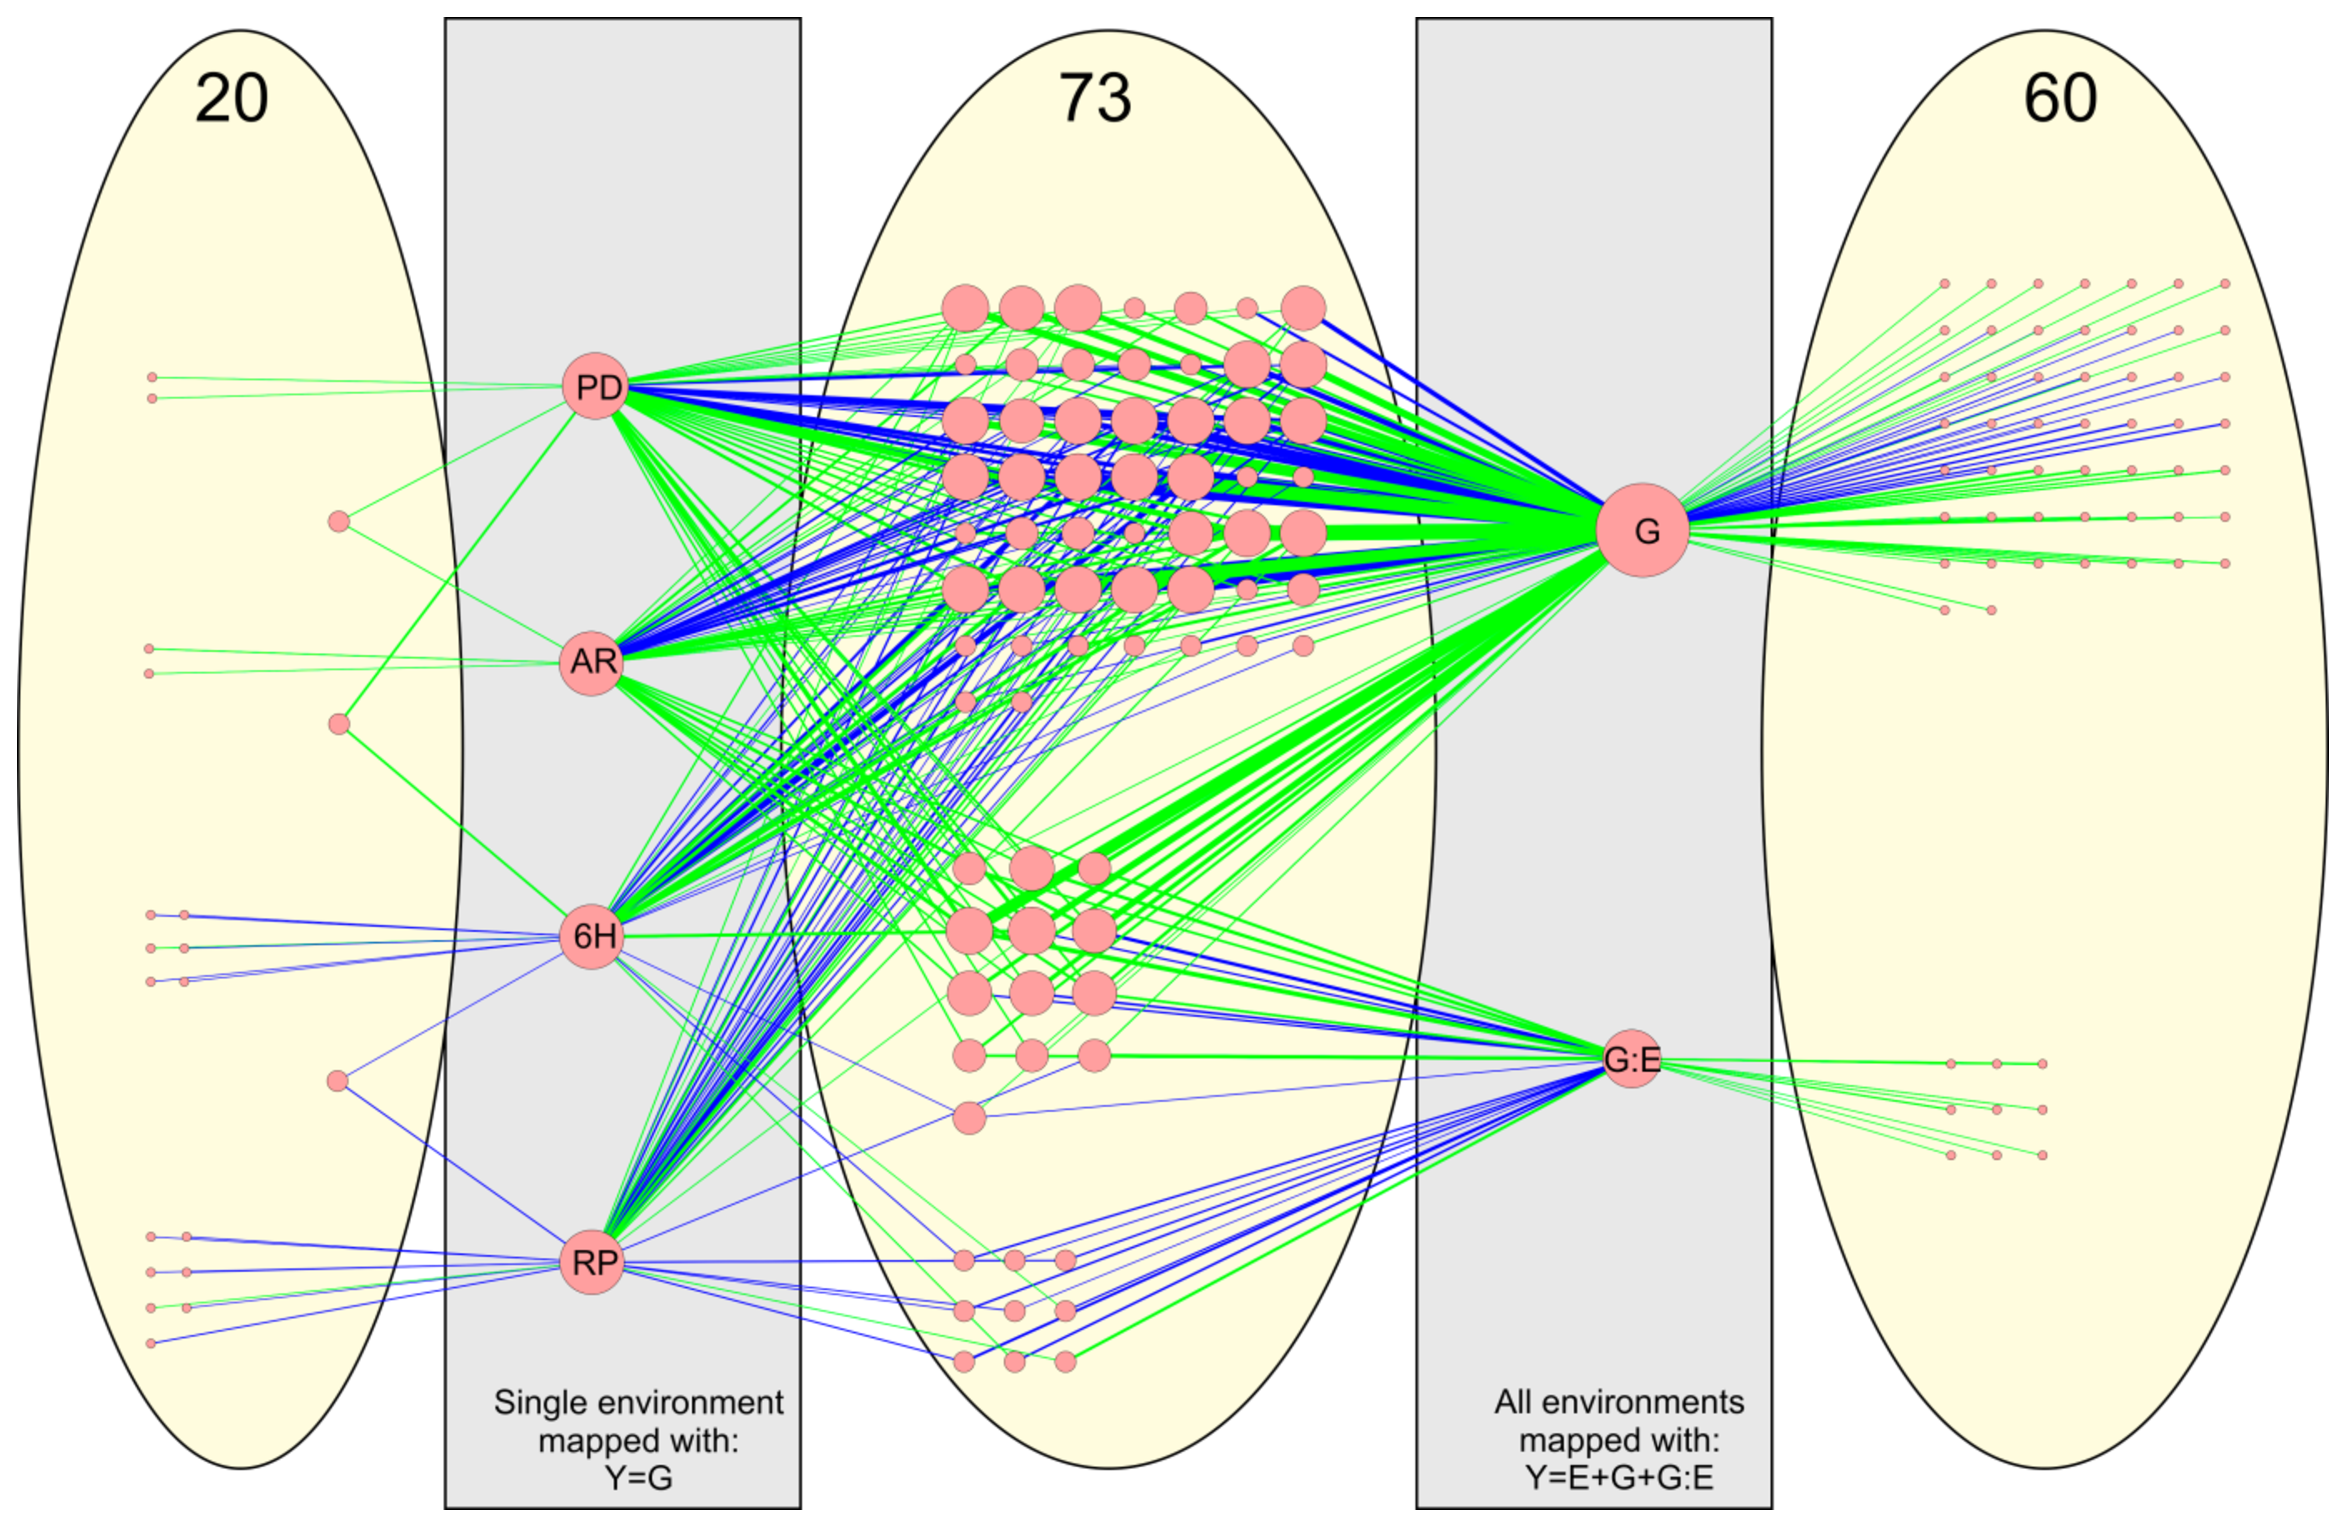
\includegraphics[keepaspectratio,scale=0.30]{eps/image_3_2_2.eps}
  \caption[Comparison of QTLs detected]{Comparison of QTLs detected within single environments (PD, AR, 
          6H and RP) by using the simple $Y=G+\epsilon$ model with QTLs detected when combining environments via the full 
          $Y=E+G+G:E+\epsilon$ model. QTLs were binned to two regions per chromosome (i.e. starting and ending regions).  
          When comparing QTLs of a single trait from two models, they are considered as shared ones if QTLs fall 
          in the same region. In total we found 73 QTLs shared between two models, as shown in the middle ellipse. 
          There are 20 and 60 QTLs that are only detected in simple and full model, respectively. Nodes indicate 
          metabolite QTLs and node size shows the degree of connectivity. Nodes are connected by edges which show 
          the link between a QTL and a mapping population (single environments versus multiple environments). 
          Separate nodes are created for the genetic (G) component and the genetic x environmental (G:E) component. 
          Edge line color represents direction of the QTLs, green for higher levels in Sha; blue for higher levels 
          in Bay-0. Edge width indicates increasing LOD scores.}
          \label{fig:qtlComparison}
\end{figure}

\subsubsection{\rev{Genetic} regulation of metabolic traits}
One of the most rewarding benefits of the generalized approach is the possibility to analyze metabolic 
fluxes over different environments or developmental stages in addition to the effect of genetic variation. 
The acquired information of both sources of variation can be effectively displayed in so-called flash cards 
in which line graphs illustrate the genetic and environmental effect and detected QTLs are plotted in heat 
bars (Fig. \ref{fig:normMetabolites}). The individual components of the linear model $Y = E + G + G:E + \epsilon$ 
provide the valuable measures for the various sources of variation. For example lysine content strongly 
increases in germinating seeds, indicated by a significant LOD score of 16.1 for the environmental effect, 
but no genetic variation for lysine could be detected (Fig. \ref{fig:normMetabolites}A). For this metabolite genetic variants vary 
indistinguishable from each other over different environments. In contrast, fumaric acid shows little variation 
between the developmental stages (LOD = 0.6), but displays strong genetic variation explained by a highly 
significant QTL (LOD 6.5) for the genetic effect at the center of chromosome II. Higher levels for fumaric
 acid are detected in all developmental stages for those lines harboring the Bay-0 allele (Fig. \ref{fig:normMetabolites}B). An 
example of the additive effect of environmental and genetic factors is the decrease in levels of malic acid 
in imbibed seeds. Here a strong environmental effect (LOD = 13.2) is accompanied with an additional genetic 
effect explained by a G QTL (LOD = 6.9) at the bottom of chromosome I. Note that the genetic effect here is 
similar in all environments (Fig. \ref{fig:normMetabolites}C). This is not the case for gluconic acid which levels are strongly 
affected by the interaction between the genotype and the environment. A strong G:E QTL (LOD = 10) is detected 
at the top of chromosome IV. The Sha allele at this position causes higher levels of gluconic acid in dry 
seeds, but not in imbibed seeds (Fig. \ref{fig:normMetabolites}D). This strong negative environmental effect (LOD = 6.6) is also 
responsible for the apparent directional shift of the G:E QTL effect.

\begin{figure}[!ht]
  \centering
  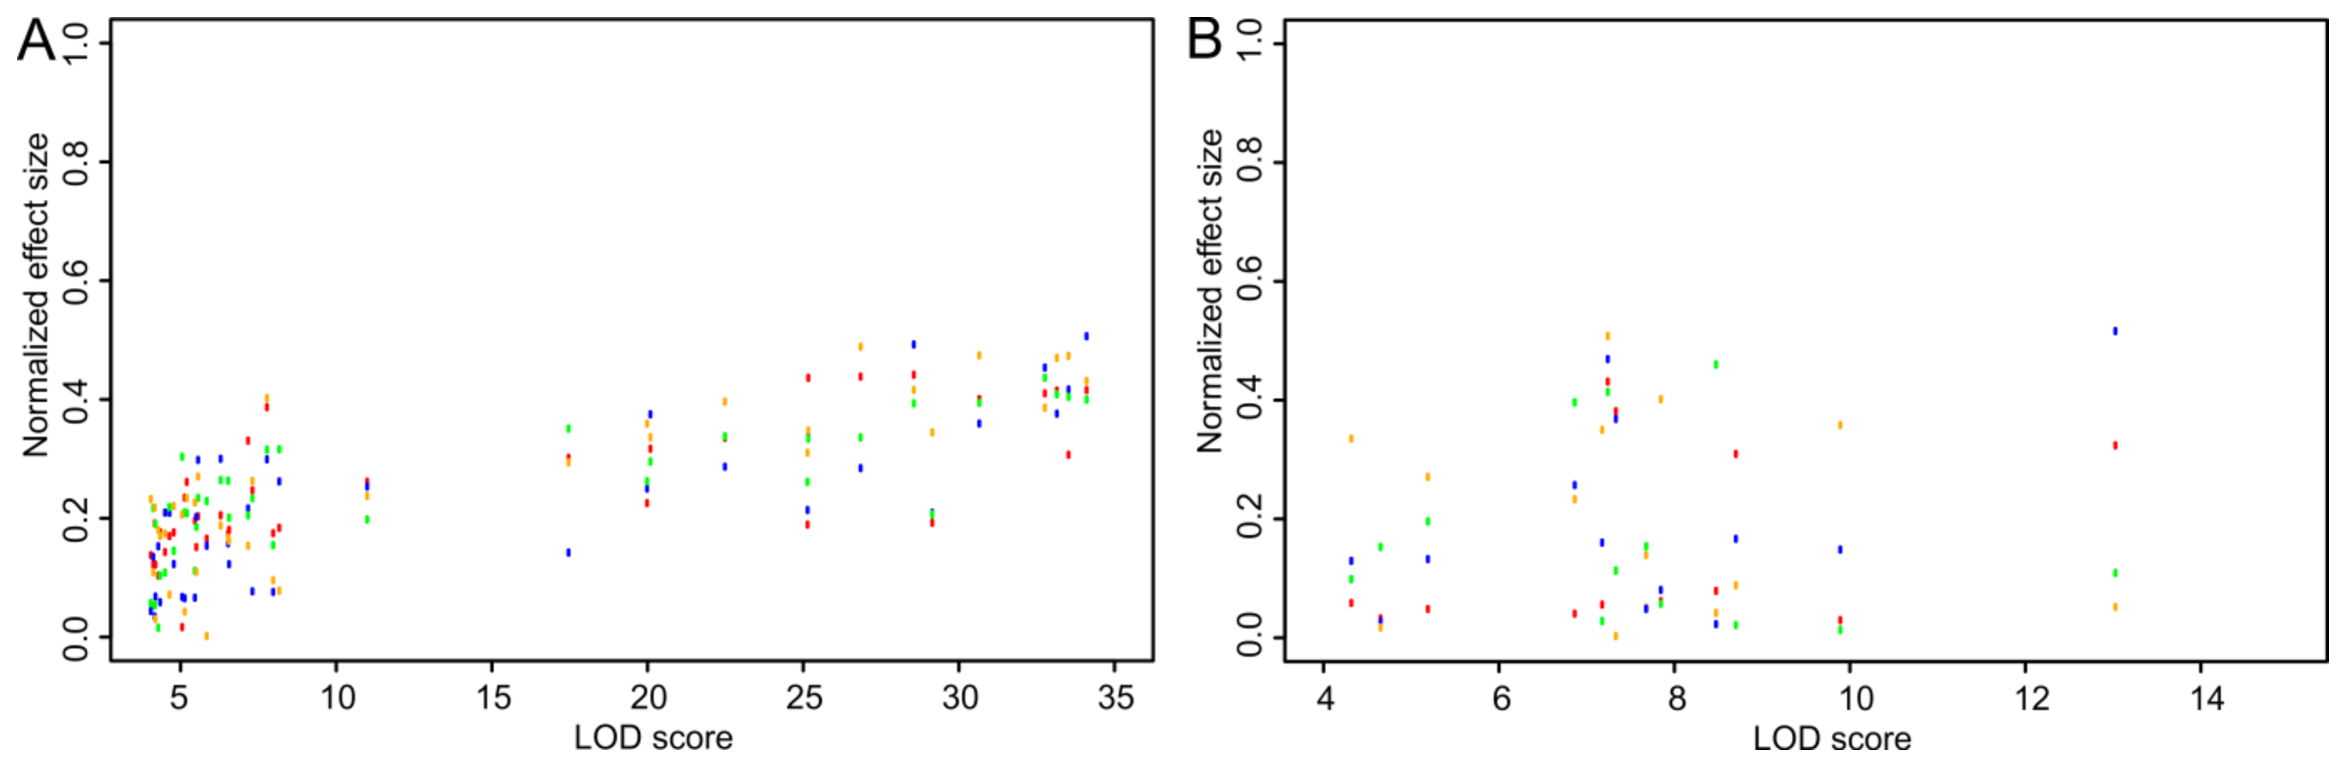
\includegraphics[keepaspectratio,scale=0.30]{eps/image_3_2_3.eps}
  \caption[Effect sizes]{Effect sizes for each individual developmental stages are plotted against the derived 
          LOD score. A: normalized allelic effect size per environment against LOD scores from the genetic (G) 
          component and B: normalized allelic effect size per environment against LOD scores from the genetic 
          x environmental interaction (G:E) component. Colors indicate the developmental stages (red = primary 
          dormant (PD); blue = after ripened (AR); green = 6 hours imbibed (6H); orange = seeds at radicle protrusion (RP).}
          \label{fig:effectSizes}
\end{figure}

Similar to the self-organizing maps in figure \ref{fig:SOM} flashcards can be instrumental in the identification of 
metabolic relationships with the added value of genetic regulatory information. This is illustrated by 
integrating flashcards of all metabolites that were identified in this study with a general Arabidopsis 
metabolic pathway diagram (\url{http://www.KEGG.jp/}). For instance, several pathways in 
carbohydrate metabolism, such as the biosynthesis routes for galactose, pentose phosphate, starch/sucrose 
and amino and nucleotide sugars, are highly interconnected and are therefore subject to co- regulation 
mechanisms. A number of compounds involved in different subparts of the carbohydrate network module (e.g. 
glucose-6-phoshate, maltose, mannose, glucuronic and gluconic acid) indeed share a strong QTL at the top 
of chromosome IV. This suggests that the observed variation for these compounds has a single genetic basis, 
possibly affecting competition for a general precursor or directing feedback loops. In addition many of 
these compounds show strong positive or negative correlation due to environmental control. Genetic 
co-regulation was also observed for amino acid metabolism. Amino acids are substrate for the synthesis of 
aminoacyl-tRNAs which in turn are essential substrates for translation \cite{Sheppard:2008}. A single 
G:E QTL at the bottom of chromosome I was detected for eight amino acids explaining a large part of the 
observed genetic variation. The joined analysis of environmentally and genetically induced variation in 
metabolic profiles can thus identify causal relationships between different modular parts of metabolic 
networks and associate these connections with relevant biological processes.

\begin{figure}[!ht]
  \centering
  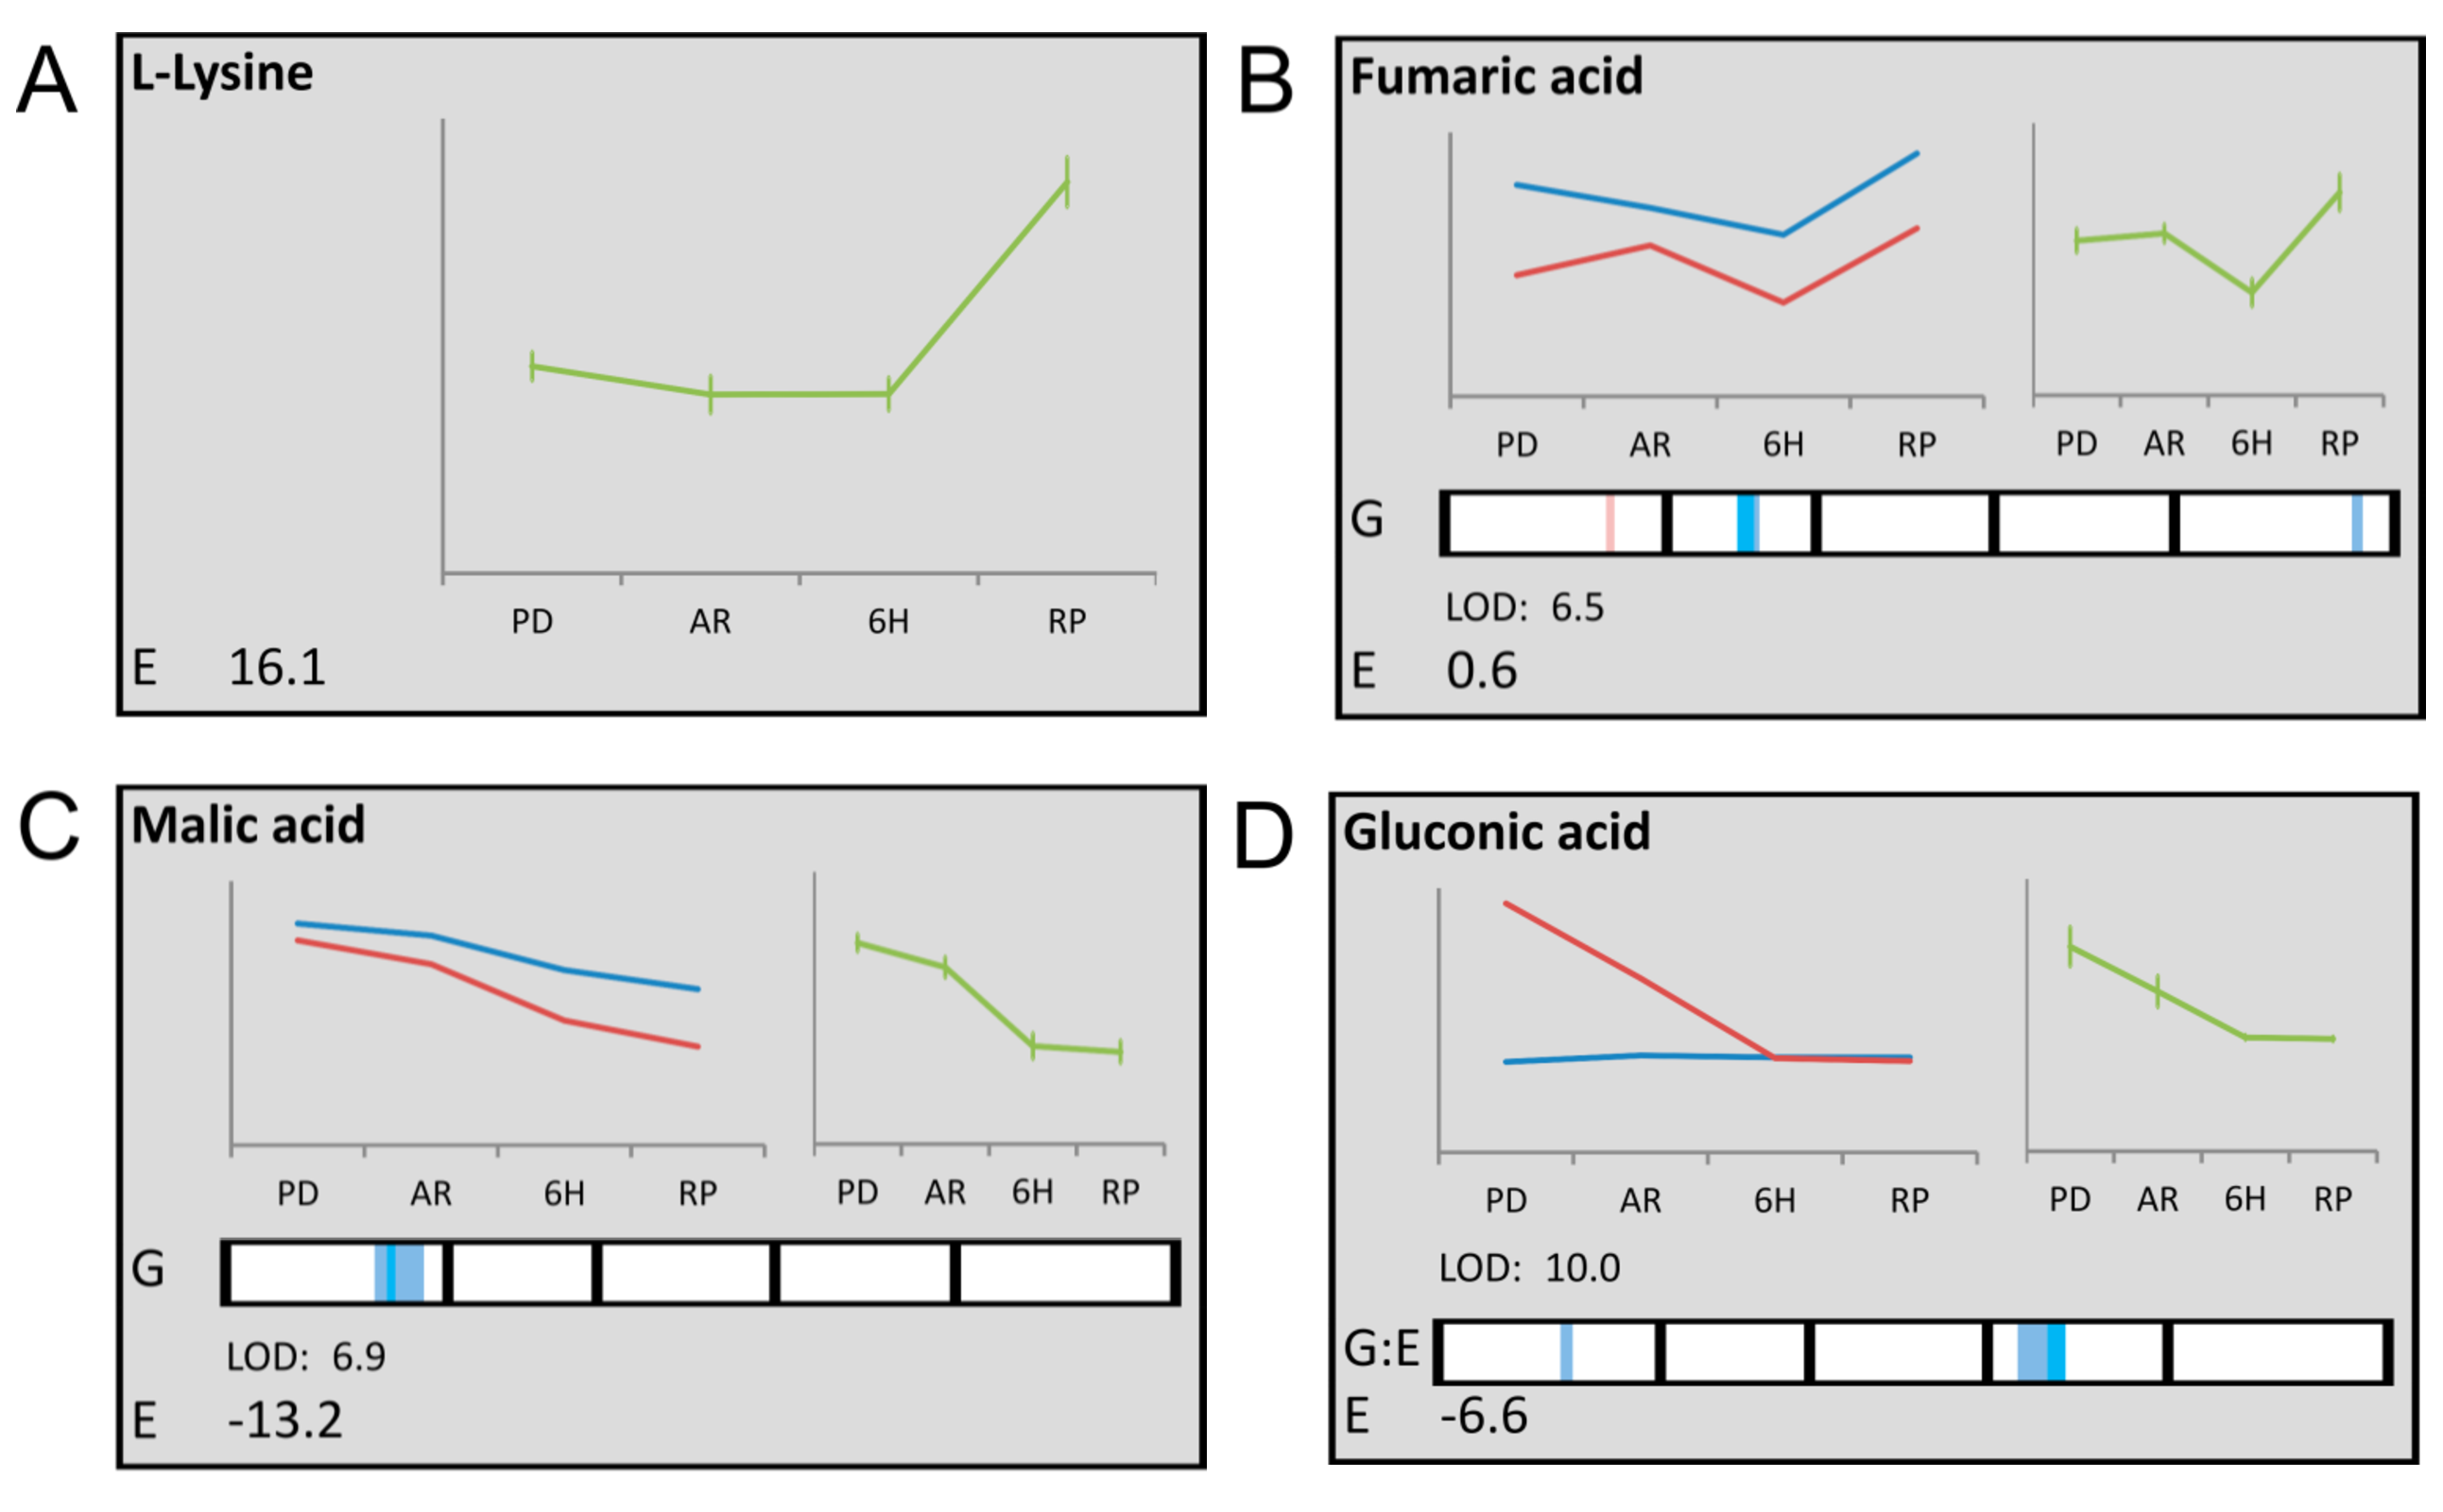
\includegraphics[keepaspectratio,scale=0.20]{eps/image_3_2_4.eps}
  \caption[Normalized metabolite changes]{Normalized metabolite changes during 4 developmental stages (PD, 
          AR, 6H and RP). Each panel represents a single metabolite and contains information about environmental 
          variation (green line plot, average over all lines within a single developmental stage) and genetic 
          variation (blue lines represent the metabolite levels for lines carrying the Bay-0 allele for the most 
          significant QTL and red lines those for the Sha allele carrying lines). QTL profiles for metabolites 
          with either genetic (G) or genetic x environmental (G:E) variation are indicated at the bottom of each 
          panel by a heat bar representing the 5 chromosomes and a false-color scale is used to indicate the QTL 
          significance. For G QTLs, positive values (light and dark blue) represent a larger effect on the metabolite 
          content for the Bay-0 allele, and negative values (light and dark red) represent a larger effect on the 
          metabolite content for the Sha allele. Interpretation of the color scale for G:E QTLs is less intuitive 
          because strong negative environmental effects can result in inversion of the QTL LOD score (e.g. gluconic acid). 
          The presented effectplot (left line plot) shows the true allele effect. Environmental (E) variation is 
          expressed as LOD score in the lower left corner. Depending on the most significant variation either, 
          genetic (G) or interaction (G:E) effects are also indicated with LOD scores in the lower left corner below 
          or above the heat bar respectively. A: L-Lysine showing only Environmental (E) variation; B: Fumaric acid: 
          showing Genetic (G) variation; C: Malic acid showing both Environmental and Genetic variation (G+E); D: 
          Gluconic acid showing interaction between Environment and Genetic variation (G:E).}
          \label{fig:normMetabolites}
\end{figure}

\subsubsection{Regulatory hotspots and physiological co-regulation}
As noted, the accumulation of several metabolites maps to identical positions suggesting that these might 
be regulated by a common genetic factor. Although co-locating QTLs can be the result of independent closely 
linked genetic factors, such coinciding QTLs are expected to occur more or less randomly by chance. Any 
deviation from expected frequency distributions along the genome thus hints at genetic co-regulation 
\cite{Breitling:2008a}. When plotted against their genomic position eight of such suggestive QTL hotspots 
can be seen (Fig. \ref{fig:nQTL}) of which the two major ones (Chromosome IV-MSAT4.8 and Chromosome V-NGA139) co-locate 
with previously identified hotspots for metabolic regulation \cite{Kliebenstein:2001, Keurentjes:2006, 
Wentzell:2007, Rowe:2008}.  Interestingly, both loci have been shown to play a role in glucosinolate 
biosynthesis. The AOP locus at chromosome IV regulates side chain modification while the 
MAM locus at chromosome V determines chain elongation, but these compounds are not targeted for in GC-MS 
analysis which predominantly detects primary metabolites. As for many glucosinolates, for some metabolites, 
including GABA and maltose, QTLs were detected at both positions. In other cases a single QTL was detected 
at chromosome IV or V, e.g. glucose-6-phosphate and tyrosine, respectively. Although the identified  primary 
metabolites are not directly connected with the glucosinolate biosynthesis pathway such associations have 
been reported before \cite{Rowe:2008}. These results might suggest alternative functions for AOP and MAM 
or a role in resource competition and allocation in central metabolism. This suggestion is further supported 
by the fact that these loci link to flowering time and the circadian clock regulation in the Bay-0 x Sha 
population \cite{Chan:2011}. It also cannot be ruled out that other genes overlapping the AOP or MAM 
regions are causal for the observed variation.

\begin{figure}[!ht]
  \centering
  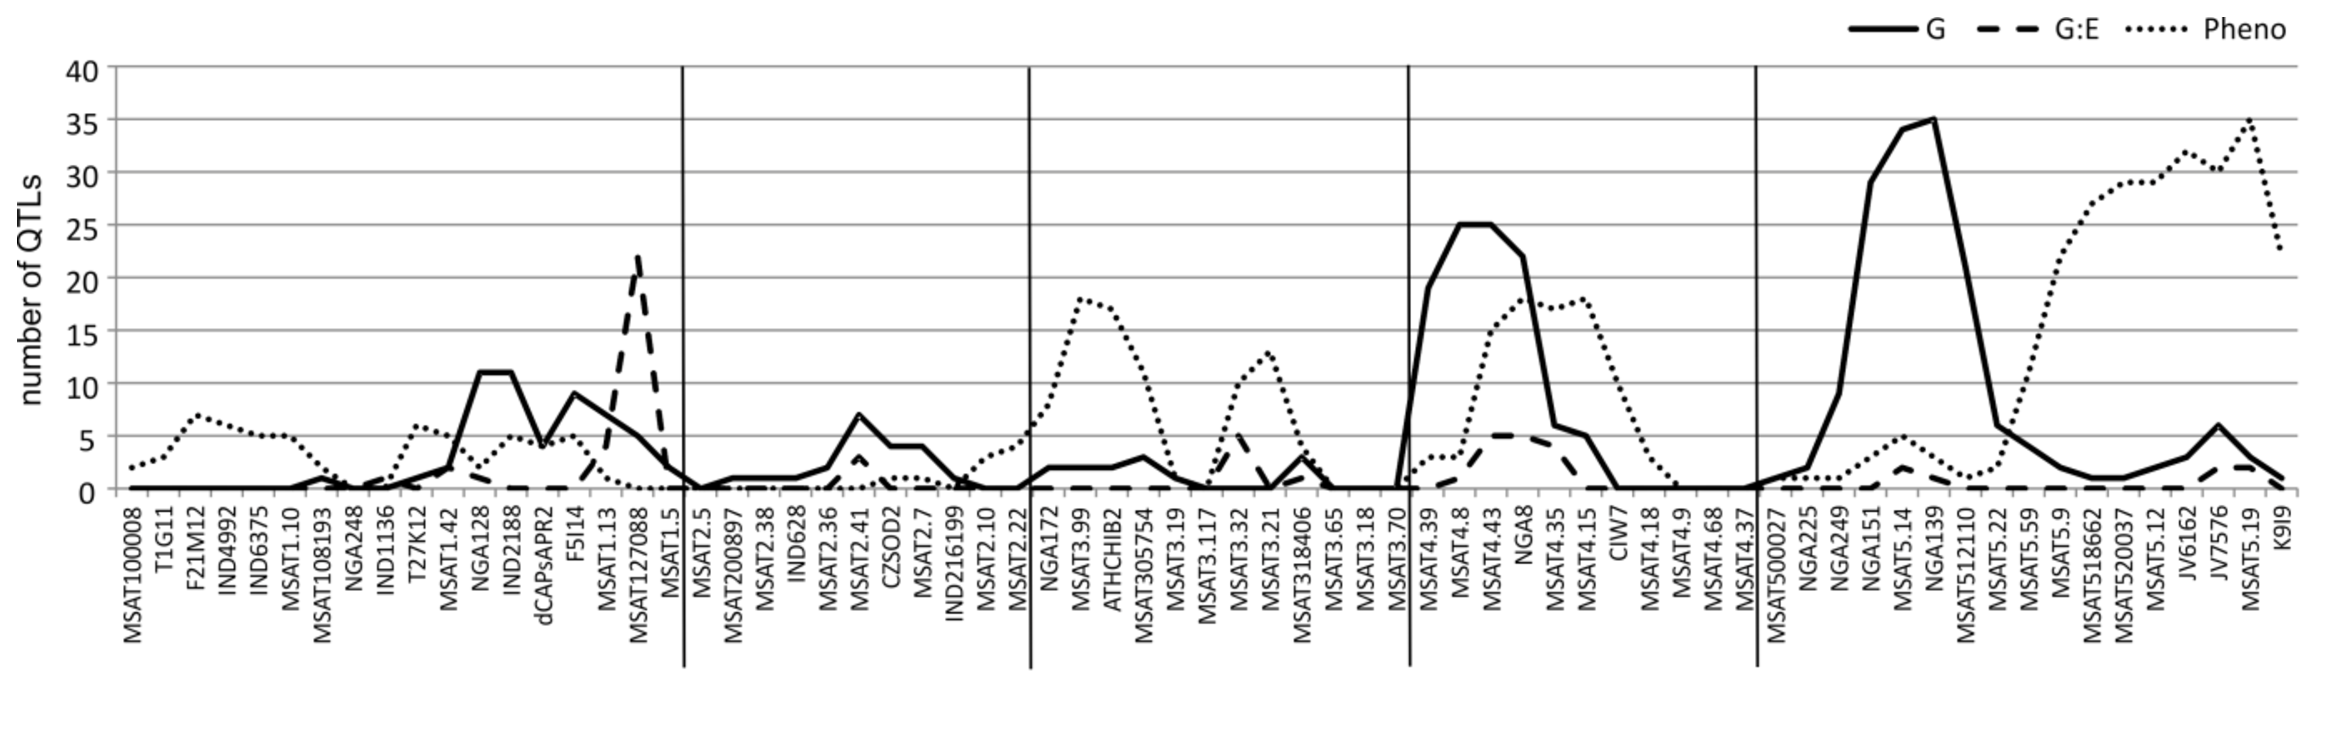
\includegraphics[keepaspectratio,scale=0.30]{eps/image_3_2_5.eps}
  \caption[Number of significant QTL]{Number of significant QTLs plotted against the genetic location. Metabolic 
          QTLs are represented by the solid (genetic component; G) and dashed (genetic x environmental component; 
          G:E) lines. Germination related QTLs \cite{Joosen:2011} are shown by the dotted line.}
          \label{fig:nQTL}
\end{figure}

Since many metabolites appear to be co-regulated, the strong impact of some loci on central metabolism might 
also exert its effect on physiological traits. Recently, the genetic landscape of seed germination in the 
same population has been described for which seed germination parameters were acquired under a wide range 
of environmental conditions \cite{Joosen:2011}. A comparison between variation in germination characteristics 
and metabolite levels might reveal compounds involved in the process of germination. Although no clear 
collocation of hotspots for germination and metabolite QTLs could be observed, incidental coincidence between 
isolated QTLs of both types of traits did occur. For instance, genetic variation for seed size co-locates 
with a large metabolic QTL cluster on the lower arm of chromosome I (~75 cM). This cluster contains many QTLs 
for amino acids, but also for components of the TCA cycle (e.g. fumarate and malate). In plants, leucine, 
isoleucine and valine, can be broken down and the end products of their catabolic pathways enter the TCA cycle 
to generate energy. It has been shown that these amino acids promote their own degradation, but only during 
seed germination, senescence, or under sugar starvation \cite{Binder:2010}. This suggests that the degradation 
pathways provide alternative carbon sources for the plant in extreme conditions. In addition, branched-chain 
amino acids and their derived alpha-keto acids are cytotoxic and preventing accumulation through degradation 

may be an important detoxification mechanism \cite{Fujiki:2000}. Higher levels of both fumarate and malate, 
as a result of the degradation of a surplus of amino acids, might thus be indicative for larger seed sizes. A 
second QTL for seed size on chromosome V co-locates with a QTL of opposite effect for GABA accumulation. 
Interestingly, Bay-0 alleles at both QTLs confer larger seed size, suggesting directed evolution (Directed 
evolution is a non-natural selection inadvertently introduced by the researchers.), as was also observed in 
a different population \cite{Alonso-Blanco:1999}. However, where levels of fumarate and malate are increased 
in larger seeds, the accumulation of GABA is decreased. GABA is known to be involved in a range of cellular 
processes \cite{Palanivelu:2003} and is rapidly accumulated in response to biotic and abiotic stresses 
\cite{Kinnersley:2000}. It has been postulated that it has roles in herbivore deterrence, pH and redox 
regulation, energy production and maintenance of carbon/nitrogen (C/N) balance \cite{Bouche:2004}. In a 
recent study, GABA levels in seeds were shown to increase by expressing glutamate decarboxylase (GAD) under a 
seed maturation-specific phaseolin promoter \cite{Fait:2011}. In accordance with our findings this resulted 
in smaller seed size and reduced seed vigor in T3 plants. No opposite seed size effect could be detected at a 
GABA QTL with increased levels due to the Bay-0 allele at the top of chromosome four, but co-locating genetic 
variation for germination on ABA, heat sensitivity and dormancy was observed at this position. These cases 
illustrate the power of joined genetic analyses of metabolic and physiological traits for the generation of 
hypotheses that can help in the functional annotation of plant metabolites and their possible role in the 
regulation of important physiological processes.

\subsubsection{Confirmation of Metabolic QTLs}
To independently confirm the effect of a single locus, it must be isolated and tested in an isogenic 
background. Several methods can be followed to perform such an independent confirmation of QTLs. A 
powerful approach is the use of residual heterozygosity in early generations of RILs. The Bay-0XSha 
RIL population(420 lines in total) was genotyped at F6, in which approximately 97\% homozygosity is 
reached in each line. This resulted in the presence of residual heterozygosity in at least a single 
RIL at almost all genome positions. Those heterozygous regions are segregating in a Mendelian fashion 
in the next generation and can be used to confirm QTL positions, as it provides a possibility to
study both parental alleles at the locus of interest in an otherwise homozygous background 
\cite{Tuinstra:1997}. In a heterogeneous inbred family (HIF), those heterozygous regions are fixed, 
and two separate lines containing the alleles of both parents, respectively, are maintained.

\begin{figure}[!ht]
  \centering
  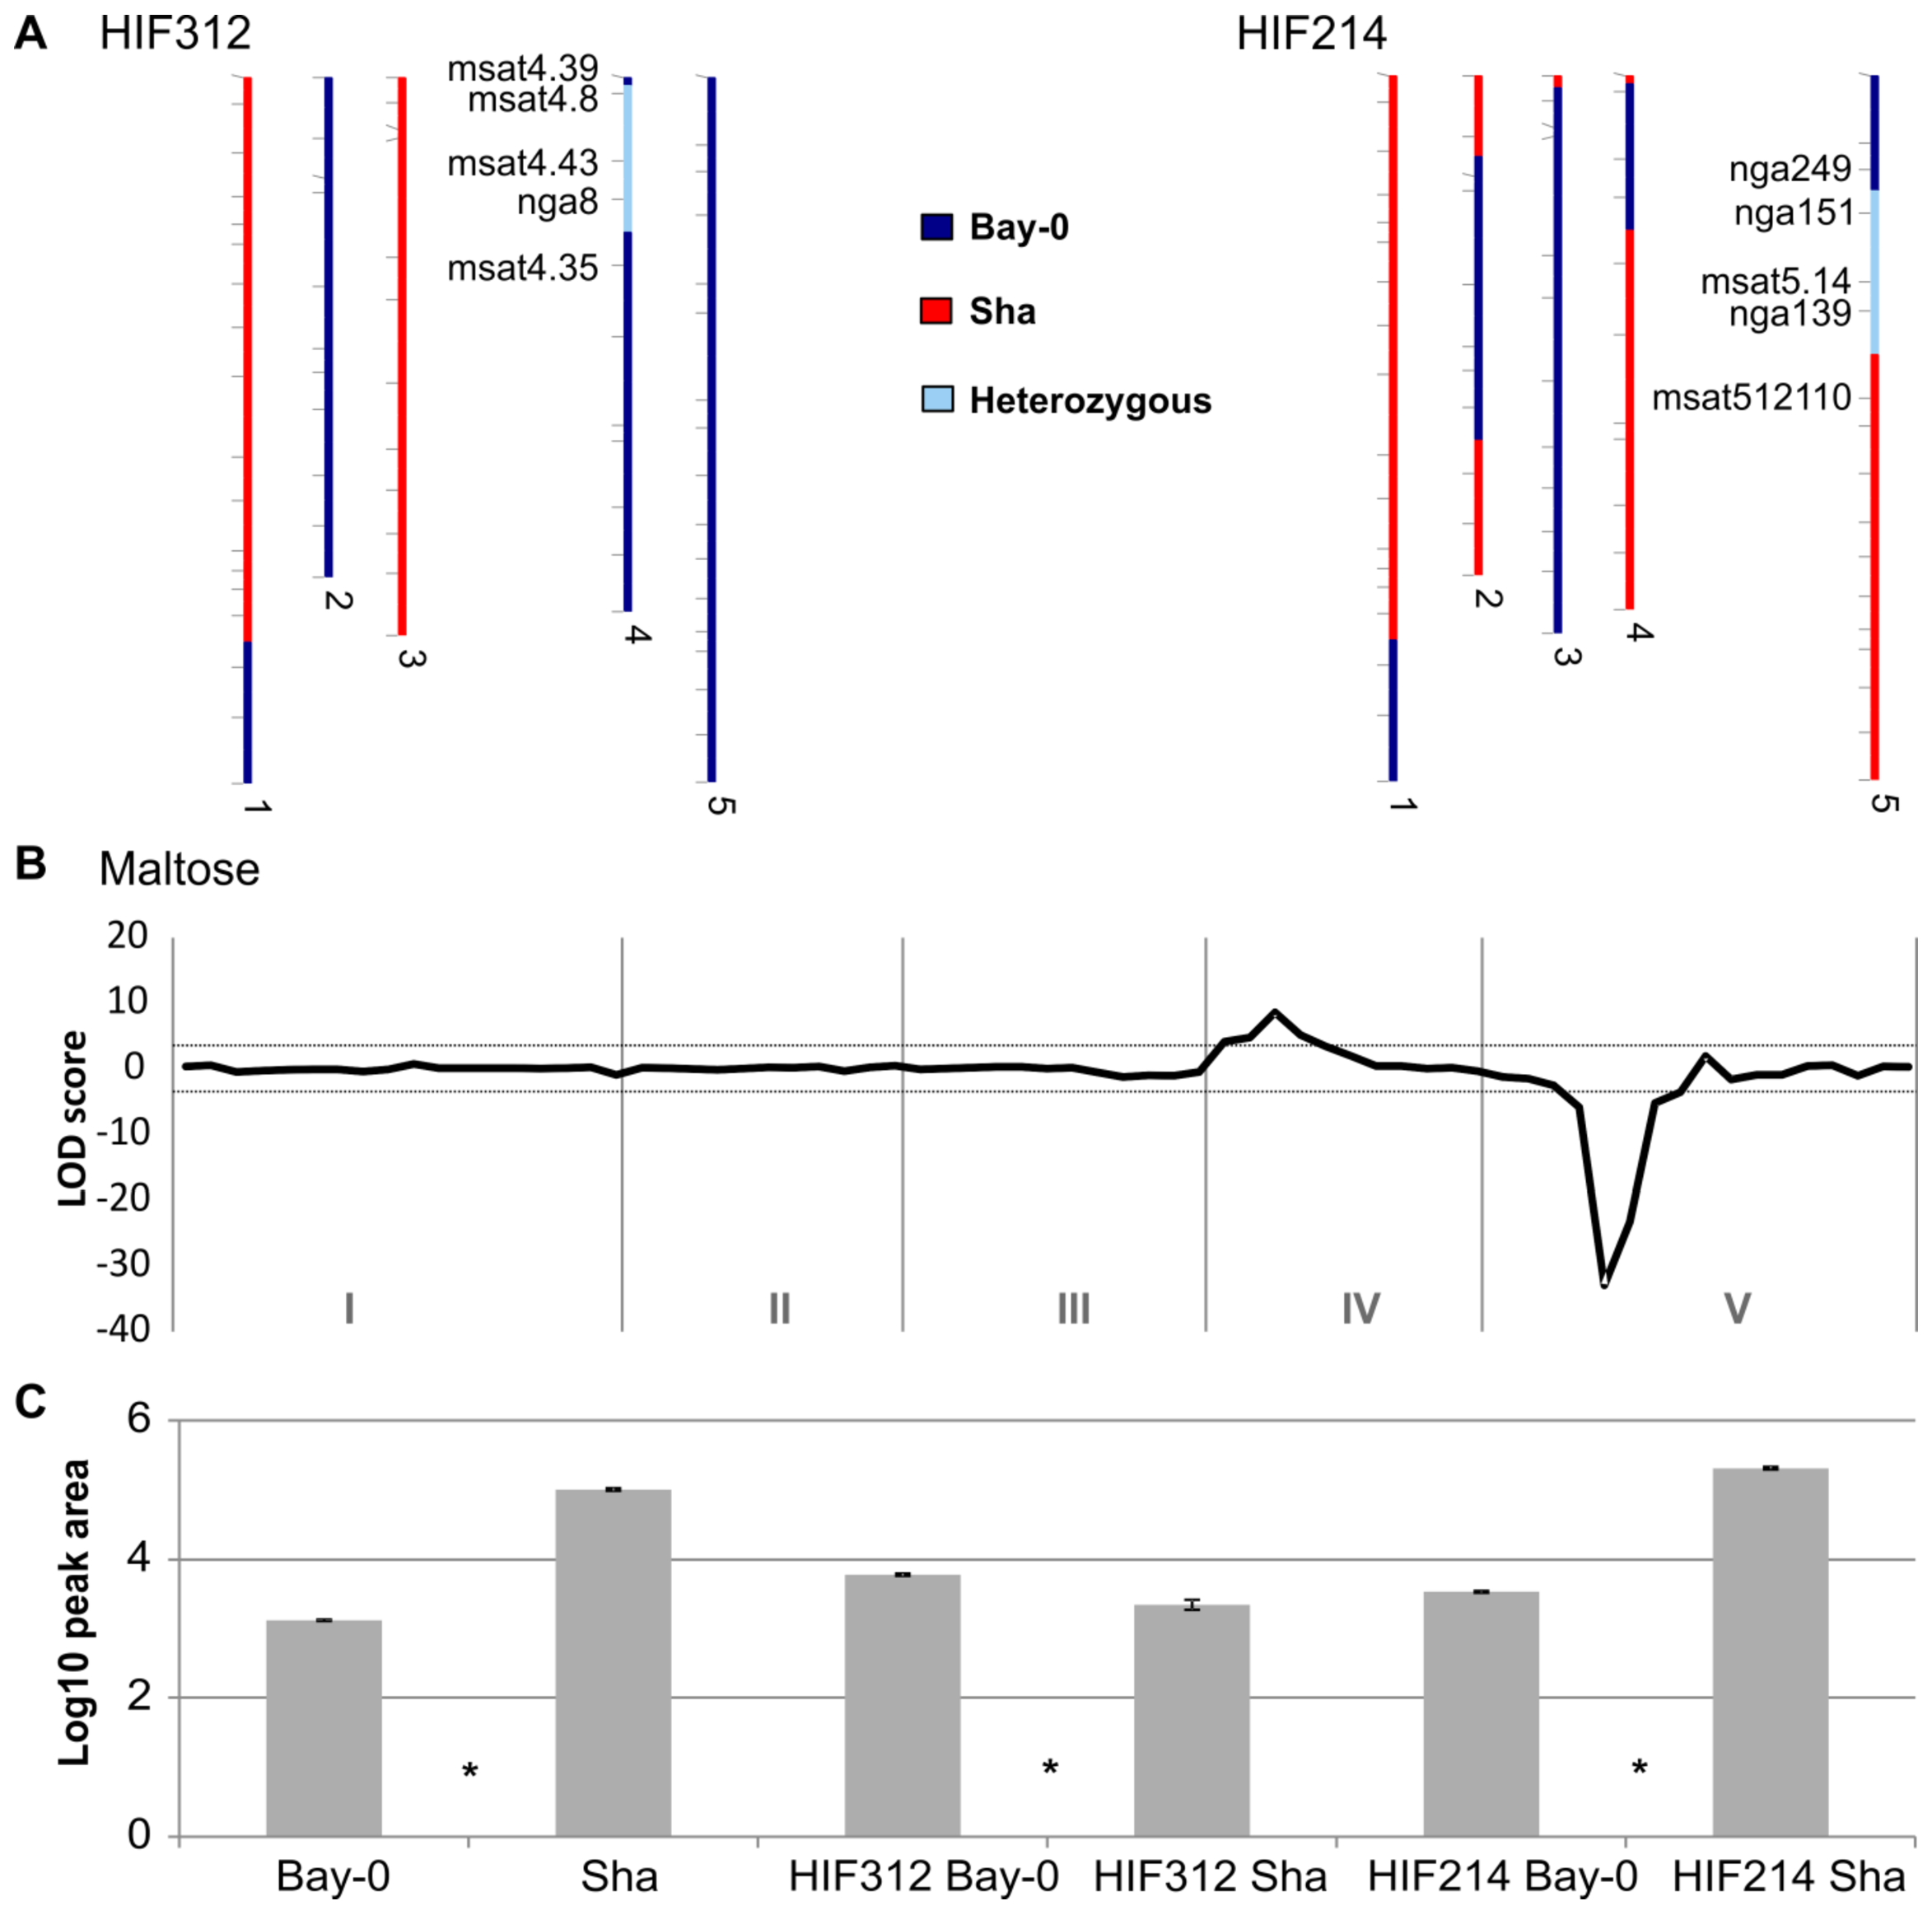
\includegraphics[keepaspectratio,scale=0.30]{eps/image_3_2_6.eps}
  \caption[QTL Confirmation]{QTL confirmation for maltose using the heterogeneous inbred family (HIF) approach. Two 
          QTL regions (top chromosome IV and top chromosome V) were analyzed using after ripened (AR) seeds of lines 
          HIF312 and HIF214 (A). The QTL profile for maltose (B) shows two significant QTLs (dashed line indicates the 
          LOD 4 significance threshold). The lower panel (C) shows the parental levels for maltose and the confirmation 
          for both QTLs by the segregating HIF lines (either fixed for Bay-0 or Sha alleles at the heterozygous interval). 
          Significant differences (t test $P < 0.05$) are indicated with * in-between the two contrasting samples..}
          \label{fig:qtlconfirmation}
\end{figure}

HIF312 and HIF214 are segregating for regions at the top of chromosomes 4 and 5 (Fig. \ref{fig:qtlconfirmation}A), respectively,
and cover the region in which the two major metabolite hotspots were detected. AR dry seeds were used to
profile the HIFs for metabolic content because many of the QTLs detected in this region showed a 
large-effect size at the dry seed stages. Significant differences between parental alleles using four 
replicates were defined by a two-tailed Student's t test($P < 0.05$). In total, 34 out of 64 QTLs could 
be confirmed using this approach. For maltose, for instance, two QTLs with 
opposite direction were found (Fig. \ref{fig:qtlconfirmation}B), which could both be confirmed using the two distinct HIFs 
(Fig. \ref{fig:qtlconfirmation}C). In a number of cases, a HIF effect was observed that was not detected significantly
in the RIL population (e.g. digalactosylglycerol). This might be the result from the higher power in 
near isogenic lines due to the absence of epistatic interactions \cite{Keurentjes:2007a}. Nonetheless, 
a substantial number of QTLs could not be confirmed by the HIF lines. The enrichment for small-effect 
QTLs in the unconfirmed class suggests that four replicates generate insufficient power to identify 
significant differences for these metabolites in the HIF experiments, although we cannot rule out that 
they are false positives from the QTL analysis. Furthermore, QTLs depending on epistatic interactions 
cannot be detected in some near-isogenic lines. In addition, a number of QTL support intervals are 
broader than the region covered by the HIF, and thus, the causal G polymorphism within the QTL interval, 
but outside the region covered by the HIF, would have been missed.

The analyses of the HIF lines indicate that most of the large-effect QTLs can be accurately detected 
using a generalized genomics approach. Although an underestimation of small-effect QTLs can be expected, 
this is largely compensated by the higher power of detecting G and E interactions

